\documentclass[a4paper,10pt]{scrartcl}
%encodings
\usepackage[utf8]{inputenc}
\usepackage[english]{babel}
\usepackage[T1]{fontenc}
%colors, hyperrefs
\usepackage{color}
\usepackage{url}
\usepackage[pdftex,pdfauthor={J\"org Behrmann, Anika Haller},pdftitle={Ma10: Auger- and Electron Energy Loss Spectroscopy}]{hyperref}
%figures and subfigures
\usepackage[pdftex]{graphicx}
\usepackage{subfigure}
%better tables
\usepackage{tabularx}
\usepackage{booktabs}
\usepackage{multirow}
%math stuff
\usepackage{amsmath}
\usepackage{amsthm}
\usepackage{amsfonts}
\usepackage{IEEEtrantools}
\usepackage[square,comma,numbers,sort&compress]{natbib}
%shiny stuff
\usepackage[babel]{microtype}
\DisableLigatures{encoding=T1,family=tt*}

\usepackage{verbatim}

\begin{document}

\title{Ma10: Auger- and Electron Energy Loss Spectroscopy}
\author{J\"org Behrmann\footnote{behrmann@physik.fu-berlin.de} \qquad Anika Haller\footnote{halleran@zedat.fu-berlin.de}}
\date{31.10.2011}
\maketitle
\tableofcontents
\thispagestyle{empty}


\section{Introduction}

In 1922 Lise Meitner first described the effect that from 1923 on would carry Pierre Augers name. For many years the features of the Auger effect were a nuissance to X-ray spectroscopists, thought to not carry any useful informations. This view has since changed in the last halfcentennial and Auger spectroscopy has thus become a very useful source of information about surface effects, due to the very short mean free path of low-energy electrons in most materials. Thus these electrons cannot penetrate the material very deeply, which makes this spectroscopic technique very surface sensitive. Furthermore, the resulting spectra are specific to the materials analyzed, therefore we will use the Auger effect in the present experiment to measure impurities on the surface of a sample and to later acertain the material of our sample.

Even for energies that cannot lead to Auger excitation electrons do scatter inelastically. The energy and deflection angle of deflected electrons can then be used to gain information about the scatterer, e.g. phonons or plasmons, with which the electron has scattered. This closely related spectroscopic technique is called Electron Energy Loss Spectroscopy (EELS) and will be usedin the our experiment to analyze surface plasmons.

\subsection{Universal Curve of Excape Depth}

Figure~\ref{fig:ucurve} shows the universal curve of electron escape depth, which shows that that the depth from which an incoming electron can escape from a surface again is only dependent on the electron's energy and thus more or less independent of the material. This universal curve can be obtained on theoretical grounds by considering that first for increasing energy (up to $70\,$eV) more and more interaction modes, e.g. phonon modes, become available as potential scatterers to the incoming electron, which decreases the particles mean free path. Whereas for even higher energies the excess energy can be used to penetrate the material further.

\begin{figure}
\centering
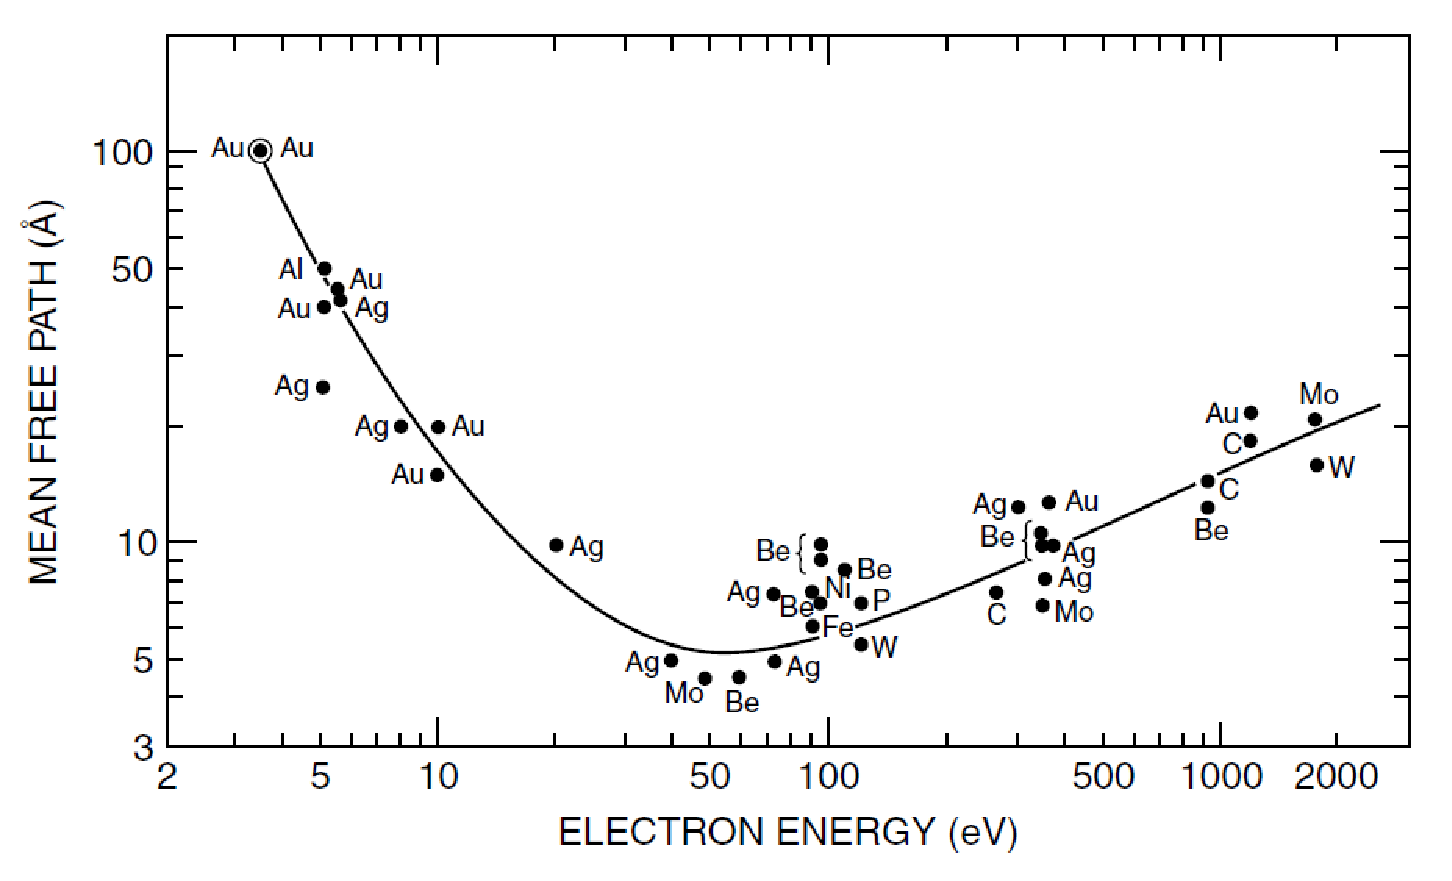
\includegraphics[scale=0.4]{img/ucurve}
\caption{Universal curve of electron escape depth \label{fig:ucurve}}
\end{figure}

\subsection{Inner-Shell Excitations and the Auger Effect}

A particle of high enough energy can scatter with an inner shell electron, exciting it enough that it leaves the atom and becomes free, leaving a hole. The atom is now in an unstable state and will relax by either by emitting an X-ray photon or an Auger electron, both possible relaxation processes are schon in~\ref{fig:aauger}.

In the X-ray relaxation process is relatively simple. An electron from a higher shell takes the place of the core electron and emits a photon in an energy range between $100\,$eV and some MeV, depending on the element. The spectrum of this process is discrete and the remaining atom is singly ionized.

The second possible relaxation process is the emission of an Auger electron. In this relaxation process an electron from a higher shell fills the core hole and the emitted photon is absorbed by another electron in a higher shell that is thus excited in the continuum. The resulting atom is doubly ionized. A schematic for the process is shown in~\ref{fig:aauger} using the example of the $KL_{1}K_L{3}$ process. The electron in the $K$-shell is excited into the continuum, an $L_1$ electron takes its place and another $l_3$ is emitted as a result.

The energy of the emitted Auger electron is given by
\begin{equation}
E_{kin} = E(K)-E(L)-E'(L') = E(K)-E(L)-E(L')-C(LL',T)+R
\end{equation}
where the $E(K)$ is the binding energy of the core electron, $E(L)$ is the binding energy of the electron filling the core hole. $E'(L')$ is the effective binding energy of the electron that is emitted as Auger electron. The effective binding energy consists of the binding energy of the shell $E(L')$, a coupling energy between the holes at $L$ and $L'$ and the final state $T$ and a so-called electronic relaxation $R$. It is important to note that the kinetic energy of the Auger electron is only dependent on the participating states of the Auger process and not on the energy of the particle that initially excites the core electron.

The dominant relaxation process is dependent on the atomic mass number $Z$, whereas for lighter atoms the relaxation by emission of an Auger electron dominates over X-ray emission.

\begin{figure}
\centering
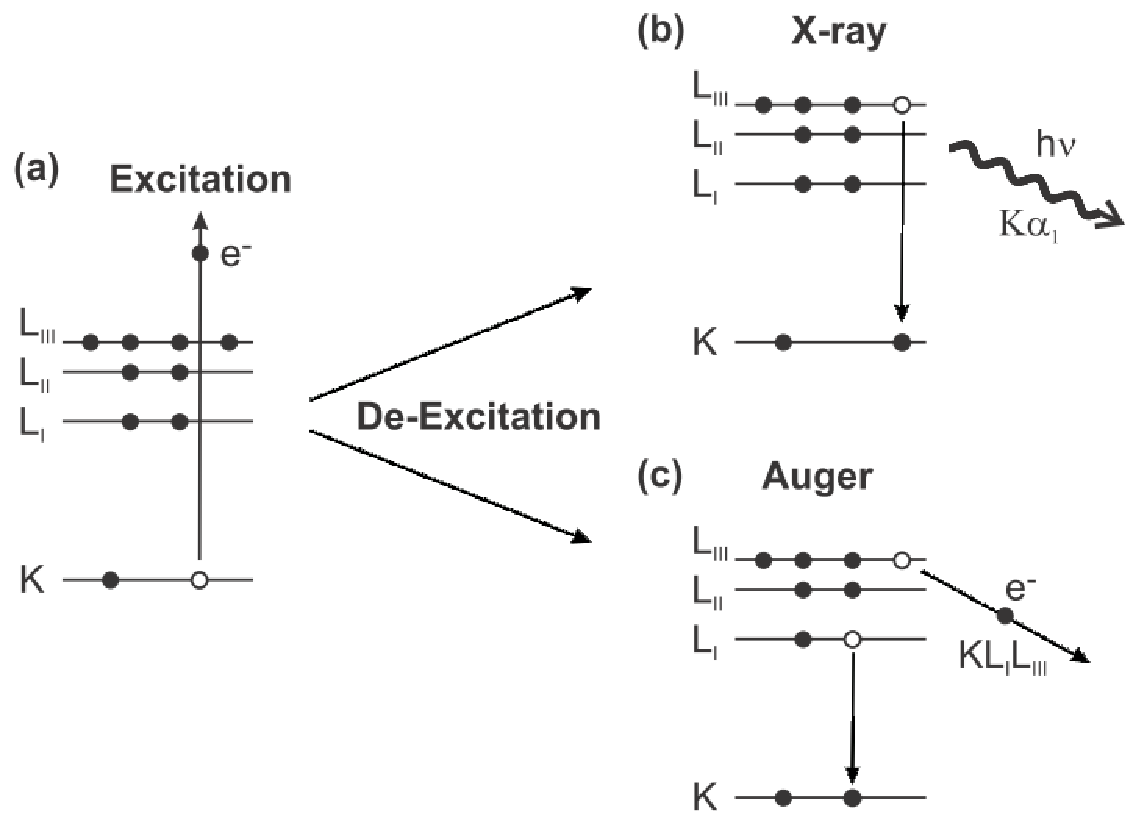
\includegraphics[scale=0.4]{img/auger}
\caption{Auger KLM process and emission of an X-ray \label{fig:aauger}}
\end{figure}


\subsection{Spin-Orbit Coupling}

To fully describe an electron's energy in an atom one has to account for magnetic moments of the electron. Each electron has a magnetic moment due to its orbital movement in the atom and another one due to its spin. All of these magnetic moments of all electrons interact and leed to energy shifts in the spectra. For light atoms the spin-orbit interaction can be approximated by an interaction of the total angular momentum and the total spin (L-S-coupling), which is possible when the coupling of individual spins and orbital angular momenta is neglible. The part of the Hamiltonian describing spin-orbit coupling is then given by
\begin{equation}
H_{SL} = - \frac{\mu_B}{\hbar m_e e c^2}\frac{1}{r}\frac{\partial V(r)}{\partial r} \boldsymbol{L}\cdot\boldsymbol{S},
\end{equation}
where $\mu_B$ is the Bohr magneton, $m_e$ is the electron mass, $e$ is the elementary charge, $c$ is the speed of light, $V$ is the core potential and $r$ is the distance of the electron to the nucleus.

For heavier atoms the coupling between individual spin and orbital momenta is nonneglible and a better approximation is the couplin of individual total angular moment $J_i=L_i+S_i$, this is called J-J-coupling.

Since Aluminum is a light element it is best described with L-S-coupling. The appropriate selection rules are thus $\Delta S=0$ and $\Delta L = 0, \pm 1$.

\subsection{X-Ray Notation}

For historical reasons X-ray notation is used in describen Auger processes. Thus the principal quantum number $n$ is represented by the letters K, L, M$\ldots$ for the numbers $1, 2, 3 \ldots$ and a subscript to those letters to associate a term symbol to those states. The states $S_{1/2}$ are given the subscript 1, $P_{1/2}$ is given the subscript 2, $P_{3/2}$ is given the subscript 3, and so on. Hence the state $L_2$ is equivalent to $2P_{1/2}$ in spectroscopic notation.

\subsection{Plasmons}

A plasmon is a quasi-particle coming up in condensed matter, describing quantized plasma oscillations, i.e. oscillations of the electron gas as a whole. The excitation energy of plasmons is specific to all materials and are given by the materials plasma frequency. For a free electron gas the bulk plasma frequency is given by
\begin{equation}
\omega_{b} = \sqrt{\frac{e^2 n}{m_e \epsilon_0}},
\end{equation}
where $e$ is the elementary charge, $\epsilon_0$ the permitivty of free space, $m_e$ the mass of the electron and $n$ the conduction electron density. 

Plasmon that appear on the interface between two materials and are confined to a surface are called surface plasmons. Because of their lower dimensionality the plasma frequence is lower than for the three-dimensional case, with $\omega_{s} = \omega_{b}/\sqrt{2}$. This excitation can be measured in the EELS part of present experiment as intensity peaks in the energy loss spectra at the energies $E=n \hbar \omega_{s}$ with $n \in \mathbb{N}$.

\section{Experimental Setup}

In this section we will describe shortly 

\subsection{Ultra High Vaccuum (UHV)}



\subsection{Cylindrical Mirror Analyzer}

\begin{figure}
\centering
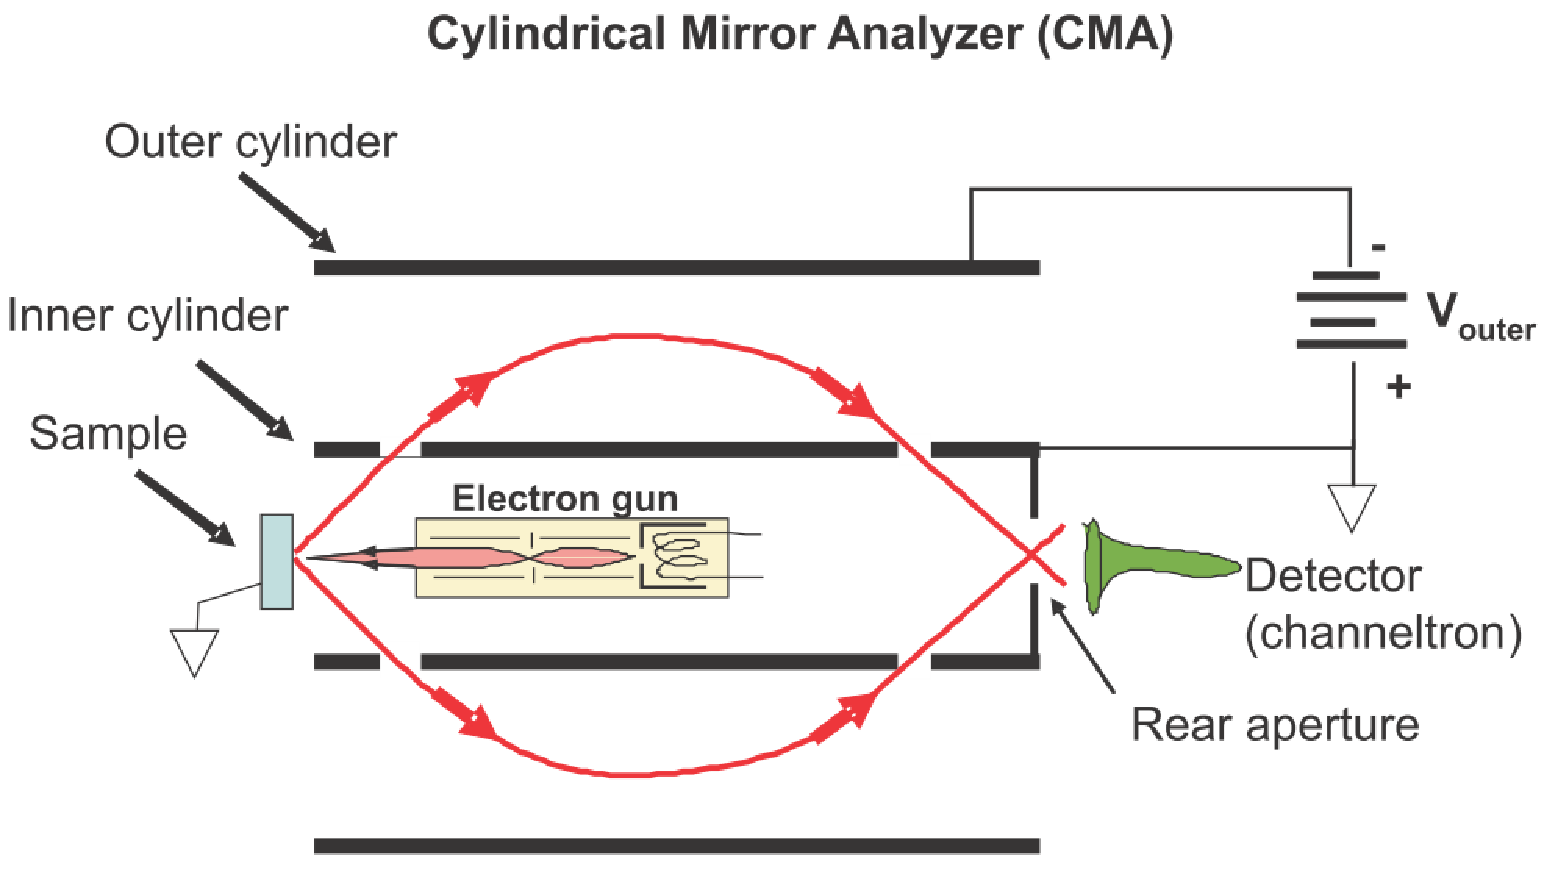
\includegraphics[scale=0.35]{img/cma}
\caption{Cylindrical mirror analyzer \label{fig:cma}}
\end{figure}


\subsection{Channeltron}

\subsection{Lock-In Amplifier}


\begin{figure}
\centering
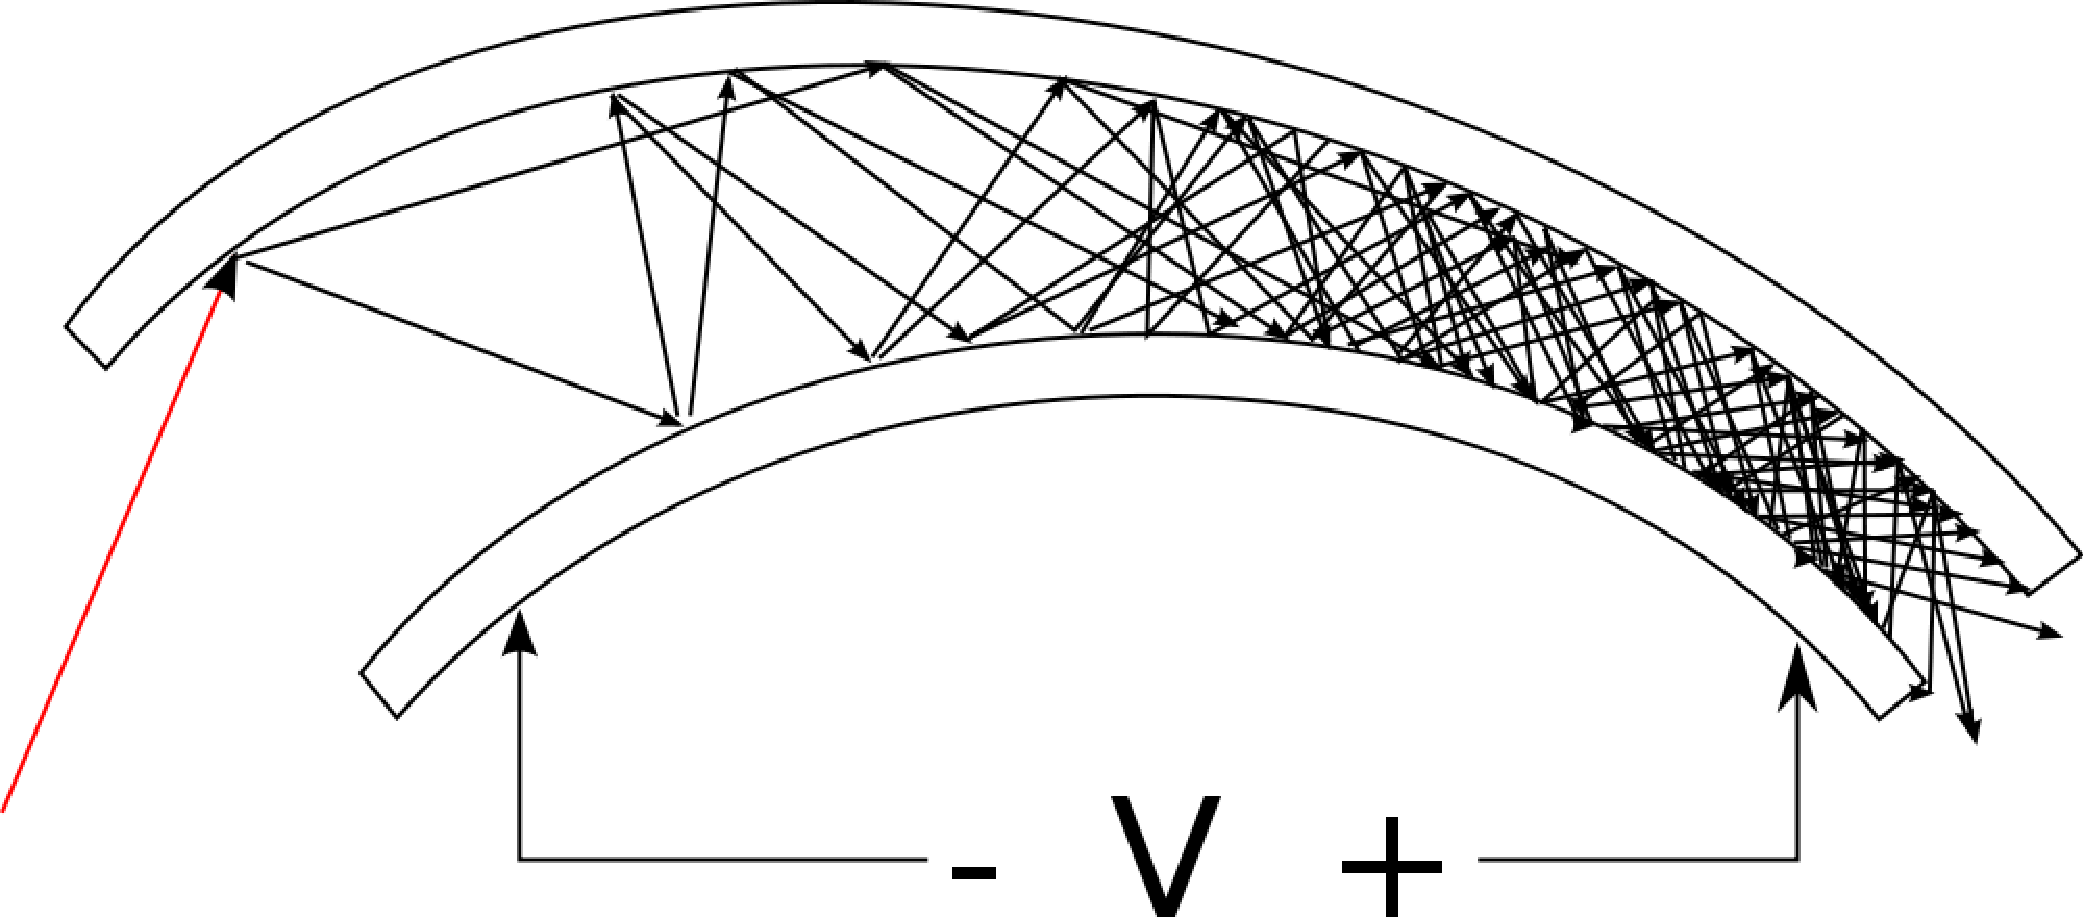
\includegraphics[scale=0.25]{img/channeltron}
\caption{Channeltronh \label{fig:ct}}
\end{figure}
\end{comment}

\end{document}
